%template for simulation report

\newpage

\section{SN1006}

\textbf{Object Description:} Large SNR (30' in diameter)

\textbf{Simulation Period:}  March 2011
% month and year

\textbf{Science Team contract:} Stephen Reynolds

\textbf{NuSIM configuration file:}

\textbf{Exposure time:} 1Ms

\textbf{Input Source:} 'Chandra mosaic.  The spectrum 
is F = 6.e-5 (E/10 keV)$^{-3.0}$ ph cm$^{-2}$ s$^{-1}$keV${^-1}$ (exactly the same as Kepler, but smeared over a much larger
object: 1\% of Kepler's surface brightness).

\textbf{Tiling Method:} 405 pointings!!!

\textbf{OA Database Version:} 007
% fill in version number e.g. 008

\textbf{Mast Bend Database:} SAA 135
% fill in SAA number

\textbf{Simulation notes:} 
% did we learn anything, did we have to do something special?

\textbf{Status:} 
% are more simulations pending? is it missing something? 

\textbf{Location and name of simulation output:} resource/examples/SN1006 in the nusim distribution on SVN

\begin{figure}[h]
\begin{center}
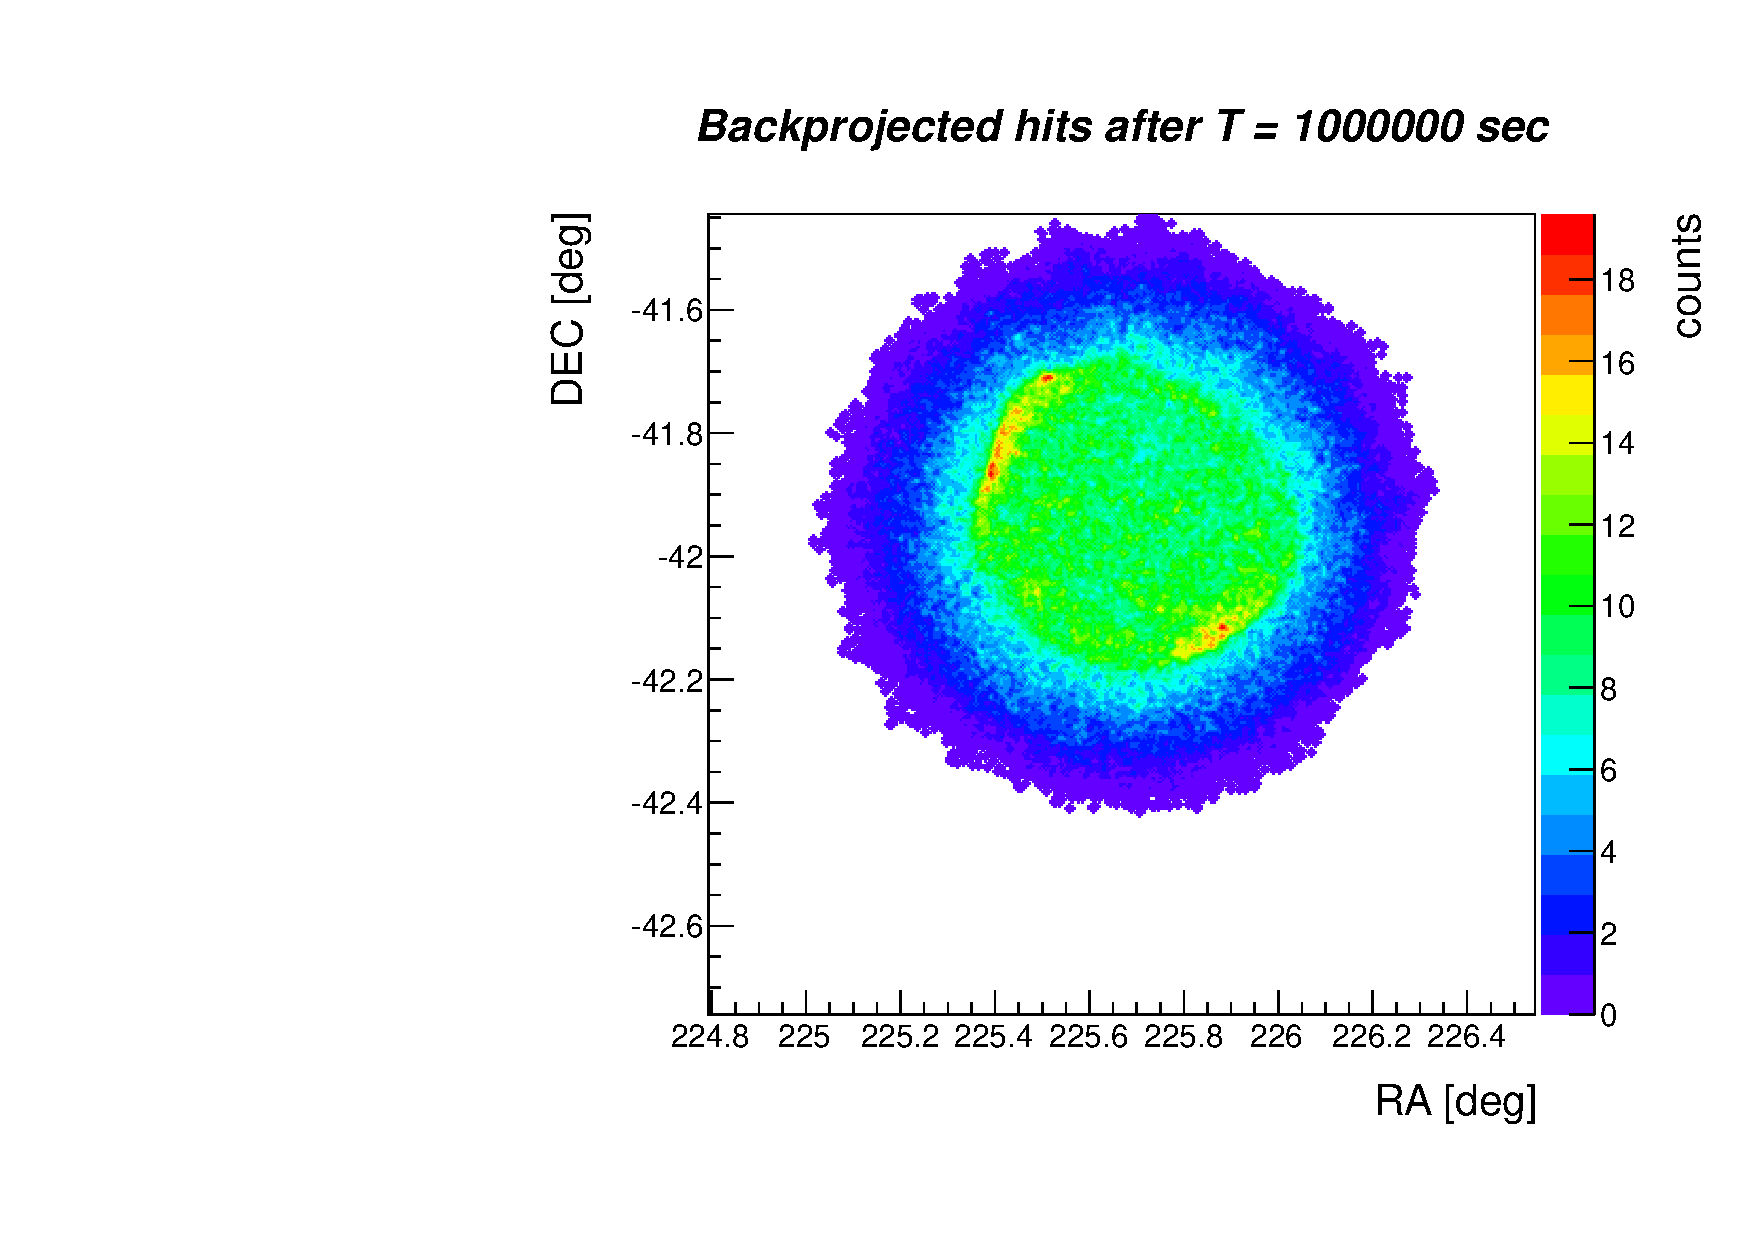
\includegraphics[width=10cm]{SN1006/SN1006.pdf}  % if there is an image put it here  
\caption{SN1006.}
\label{sn1006} 
\end{center}
\end{figure}

